\chapter{Particles}

\begin{figure}
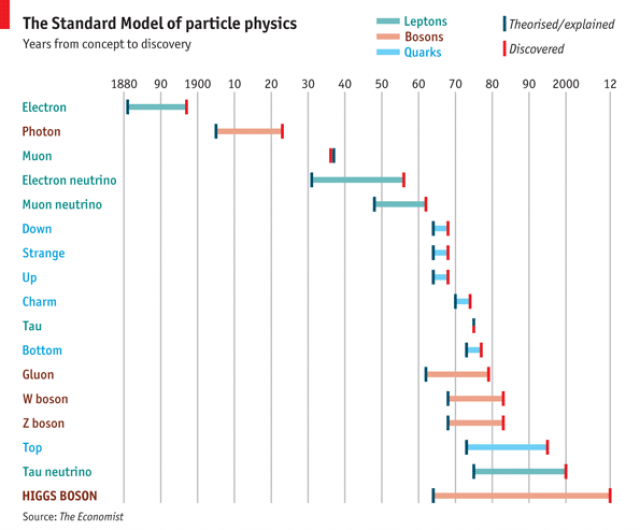
\includegraphics[width=\textwidth]{physics/images/particle_timeline}
\caption{Timeline of particle theorization and discovery}
\end{figure}
Mass difference between initial particle and decay products is the primary factor determining lifetime (smaller the difference, longer the lifetime). When looking at a decay, one can get an idea of the amplitude by multiplying the coulpling constant $g$ for each vertex with that coupling, and $1/(q^2 - m^2)$ for each internal line, where $m$ is the internal line particle.

Nobody chooses to name new particles $\iota$ (iota) since it has a connotation of insignificance.




\section{Leptons}
\subsection{Electron}

\subsection{Muon}

Muons have a lifetime of $10^{-6}$ s, and decay to electrons (with a pair of neutrinos to conserve Lepton number). The have a mass of 105 MeV, about a tenth that of the proton.

Muon does not decay to an electron via photon

Prompt muon decays from $W,Z$ decay.

\subsection{Tau}
Mass of 1.776 GeV and a lifetime of $10^{-13}$. Decay hadronically (mostly to pions) $65\%$ of the time.

\subsection{Neutrino}\label{neutrino}
Looking at products of neutron decay 
\begin{align}
n\rightarrow p^+ + e^-+ \nu_{\bar{e}}
\end{align}
the momentum of the proton and electron is not always back to back. Pauli posited the existence of another particle to save four-momentum conservation. We know it is there because...

Neutrinos are detected after they interact weakly with some material, through exchange of a $W$ or $Z$. The flavor of the neutrino is deduced because after $W$ exchange, you have the corresponding lepton. With that lepton, you can tell what it is from Cherenkov radiation if it is relativistic.

Majorana fermions are their own antiparticle, which neutrinos might be.

\section{Quarks}
Quarks compose Hadrons which is a super group of Mesons (quark-antiquark pair) and Baryons (three quarks).
\begin{itemize}
    \item $u$ - The up quark is the lightest of all the quarks with a mass of only 2.3 MeV, about 4 electrons.
    \item $d$ - The down quark is the second lightest quark with a mass of 4.8 MeV.
    \item $c$ - The charm quark has a mass of 1.29 GeV is the third largest quark, just larger than a proton.
    \item $s$ - The strange quark is the third lightest quark with a mass of only 95 MeV, roughly a muon. Was theorized by Murray Gell-Mann, and found at SLAC in 1968.
    \item $t$ - The top quark is the heaviest quark at 175 GeV, about the size of a tungsten atom. Since it is so heavy it decays with a lifetime of just $10^{-25}s$, which is short than the lifetime of the strong interaction, preventing it from forming hadrons. The only way a single quark can decay is through a $W$ boson, which makes $t\rightarrow Wb$ happen $99.8\%$ of the time. It was postulated in 1973 and found in 1995 at CDF at Fermilab.
    \item $b$ - The bottom quark has a mass of 4.18 GeV, the second largest quark. CKM matrix elements $V_{ub}$ and $V_{cb}$ are suppressed making the lifetime long $10^{-12}$ s. Mesons made of $b$ quarks have algorithms for identification within CMS due from their long lifetime (Section \ref{id-aglos}).
\end{itemize}

\section{Mesons}
Mesons contain both a quark and antiquark pair.

\subsection{Pion}
There are two types of pions charged and uncharged. Each have a mass of roughly 140 MeV, making them a bit larger than a muon. Both have Spin-0
\begin{itemize}
    \item $\pi^+ = u\bar{d}$, $\pi^- = d\bar{u}$. Charged pions mostly ($99.99\%$ of the time) decay weakly to $\mu, \nu_\mu$ with a lifetime of $10^{-8}$ s.
    \item $\pi^0 = u\bar{u}, d\bar{d}$. Mostly ($98.82\%$ of the time) decay electromagnetically to a pair of photons with a shorter lifetime of $10^{-13}$ s
\end{itemize}
Hideki Yukawa in 1935 originally predicted the existence of mesons as the carrier particles of the strong force, which the muon was mistaken to be a year later.

\subsection{$J/\Psi$}

The $J/\Psi = c\bar{c}$ has a mass of 3.1 GeV, about the mass of tritium. The name comes from the near simultaneous discovery in 1974 from both Burton Richter at SLAC ($\Psi$) and Samuel Ting at Brookhaven National Lab ($J$). The lifetime is $10^{-20}$ s, which is very long, since it mostly decays strongly ($10^{-23}$ s). The long lifetime is due to toe OZI Rule (Section \ref{ozi}). $6\%$ branching ratio to muons

\subsection{Kaon}
The Kaon is $K^+ = u\bar{s}, K^0 =( d\bar{s}, \bar{s}d), K^- = \bar{u}s$ and has a mass of 493 MeV, about 5 muons. $64\%$ of charged Kaon's decay to muons.

\section{Baryons}
Baryons contain three quarks

\subsection{Proton}
Proton is the lightest Baryon which prevents it from decay from conservation of Baryon number.

\subsection{Neutron}

A neutron is composed of two down quarks and one up quark making it a "$dud$". 
Lifetime of 15 minutes. Produced in collisions(?), only slowed down through bumping into things of roughly equal size. If it hits a proton, the proton showers and is how the neutron eventually loses energy. The neutron will slow down until it reaches thermal energy of about $1/40 eV$. It then gets absorbed by a nucleus(?) which gives of ~MeV photons, which can then pair produce and make electrons where they shouldn't be. 


\section{Bosons}
\subsection{$W$ Boson}

Mass of 80 GeV. Decays can be found with counting arguments, allowed decays are $e\nu_e, \mu\nu_\mu,\tau\nu_\tau, ud, sc$. The combination $tb$ is not allowed since the $t$ is so heavy. The color combinations make each quark combination have 3 possibilities. Thus if we want to know the branching ratio to $e\nu_e$

\begin{align}
B(W\rightarrow e\nu) = \frac{1}{1+1+1+3+3} = \frac{1}{9}\approx 11\%
\end{align}

\subsection{$Z$ Boson}

Mass of 91 GeV. Can't use the same counting arguments we used for the $W$ because there is different coupling for different fermions. The width of the $Z$ boson is dependent on the number of possile final states into which it can decay, so the measurement of the width is a good probe into the existence of a fourth generation of leptons\cite{bstone}. The relationship between the width and decay modes is as follows:
\begin{itemize}
    \item The uncertainty principle gives us a rule of thumb to relate energy width and time
    \begin{align}
    \Delta E\Delta t\ge \hbar/2
    \end{align}
    According to Bob Cousins, this is the wrong way to think about it, but it is no doubt much easier to remember.
    \item The mean lifetime $\tau$ of the $Z$ is related to it's decay constant $\Gamma$ through
    \begin{align}
    \tau = \frac{1}{\Gamma}
    \end{align}
    \item Putting these two together, we see
    \begin{align}
    \Gamma \propto \Delta E
    \end{align}
    \item Since the decay constant is additive
    \begin{align}
    \Gamma = \Gamma_{ee} + \Gamma_{\mu\mu} + \Gamma_{\nu\nu} +  \ldots
    \end{align}
    We see that if we add another decay channel to the $Z$, we increase the width of the mass itself.
\end{itemize}
The height is proportional to $\frac{\Gamma(Z\rightarrow hadrons)}{\Gamma(Z\rightarrow all)}$ so if there are more leptons, the height will also be reduced. These type of measurements were what LEP (Section \ref{lep}) was used for.

\subsection{Higgs}


\begin{figure}
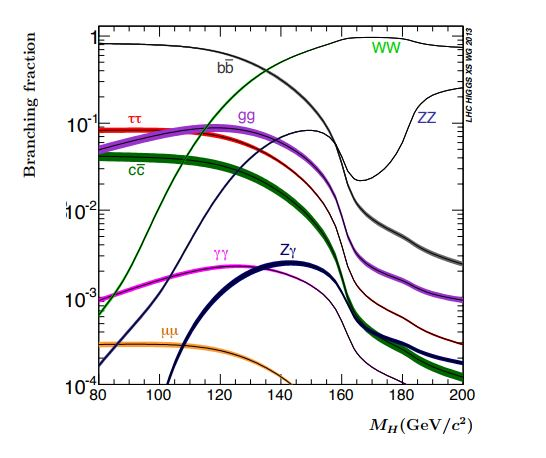
\includegraphics[width=\textwidth]{physics/images/higgs_br.jpg}
\caption{Branching fraction of Highs boson as a function of mass. Fraction to $WW$ is higher than to $ZZ$ at higher $m_H$ due to $Z$'s being identical particles. The branching ratio is exactly a factor of 2 at high mass.}
\end{figure}


With a mass of 125 GeV, the Higgs was the most recent elementary particle to be discovered and was the lynchpin of the Standard Model. Higgs not discovered in earlier colliders because:
\begin{itemize}
    \item Too low center of mass energy
    \item $ee$ collider has small cross-section to Higgs, since coupling is proportional to mass of particle.  $u$ and $d$ are also very light, so also not a great candidates. Need high energy $g$ to make a pair of $t\bar{t}$ to make a $h$
\end{itemize}
Higgs production in proton-proton collisions proceeds in one of four ways:
\begin{enumerate}[label=(\alph*)]
    \item Gluon Fusion, in which two gluons interact via a loop of QCD fermions (top is largest contribution) to produce a single Higgs boson
    
    \item Vector Boson Fusion, in which two quarks radiate a weak boson which fuse and couple directly to a Higgs. This Higgs is produced in association with two jets.
    
    \item Higgs-strahlung, in which a gauge boson produced in the pp collision radiates a Higgs. This Higgs is thus produced in association with the gauge boson.
    
    \item Associated top quark pair production.
\end{enumerate} 

At current LHC energies, $\sqrt{s} = 13 \text{ TeV}$, gluons carry most of the proton's momentum and so Gluon Fusion is the dominant production mechanism, followed by VBF. Below are Feynman diagrams to LO for these production mechanisms:

\begin{center}
    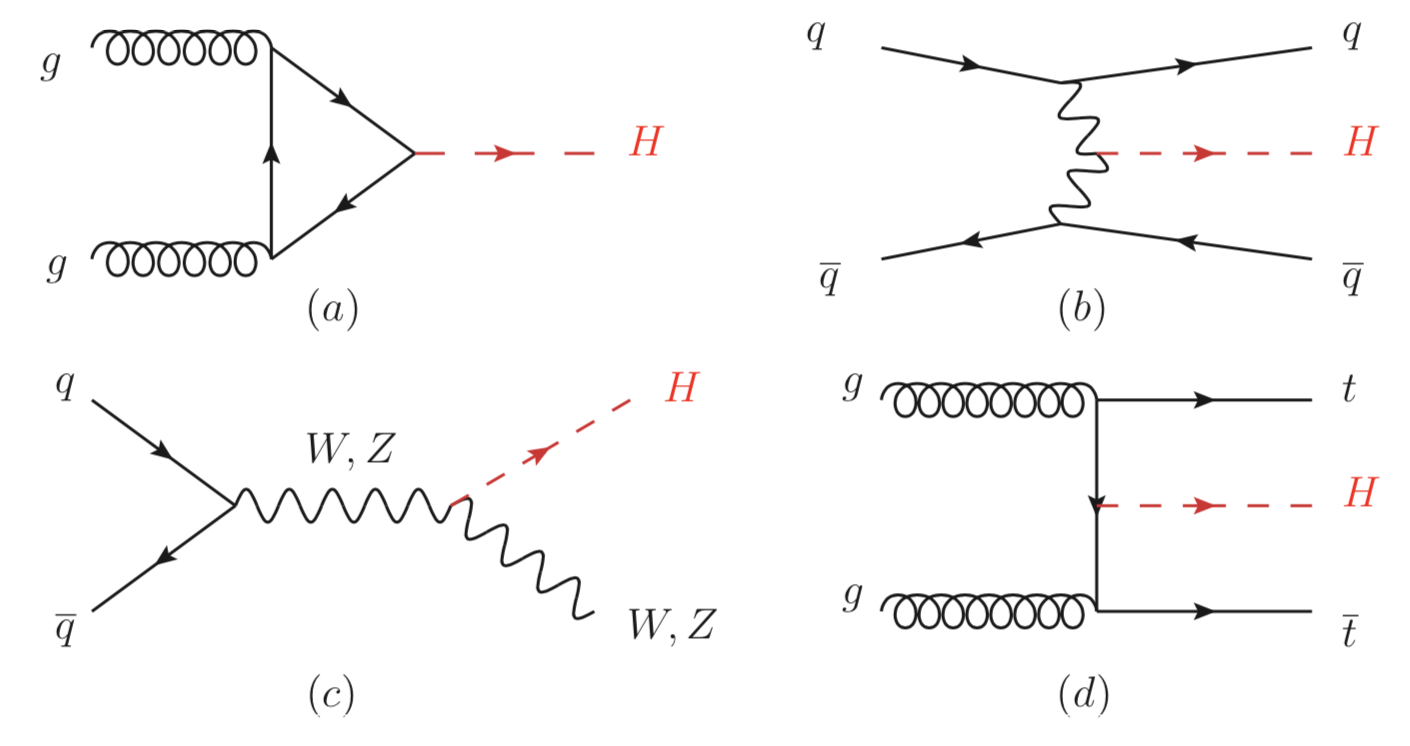
\includegraphics[scale=0.5]{physics/images/higgs_production_diagrams}
\end{center}

While GF dominates Higgs production at LHC energies, other production mechanisms are still important for Higgs analysis. Consider VBF, where the scattered quarks manifest into two hard jets appearing in the forward and backward regions of the detector. Because of the color-singlet nature of the weak-boson exchange, gluon radiation from the central rapidity regions is strongly suppressed. This feature can be exploited to reduce overwhelming QCD backgrounds, including GF-induced Higgs + 2-jet production or $VH$ production with hadronically decaying weak-boson. Thus VBF is valuable as a clean environment for Higgs searches and measurements of Higgs couplings. A typical VBF event includes a Higgs candidate accompanied by two energetic jets ($\geq 30 \text{ GeV}$), with a large dijet mass ($m_{jj} \geq 400\text{ GeV}$) and pseuodrapidity ($\Delta\eta_{jj} \geq 3.5$). However, such a sample does have contamination from GF-produced Higgs.

$VH$ production follows VBF in importance at the LHC, seen primarily as Higgs-strahlung but also in a diagram without a virtual weak boson, in which $ZH$ couples to gluons via a top-quark loop. $VH$ production, together with $t\overline{t}H$ production, provides a relatively clean environment to study Higgs decays into $b$ quarks.

\vspace{1em}
\vspace{1em}
There are five main sets of Higgs final states for which there are searches at the LHC: $b\overline{b}$, $W^+W^-$, $ZZ$, $\gamma \gamma$, and $\tau^+\tau^-$. The following table summarizes the theoretical cross sections for modes of Higgs production and decays:

\begin{center}
    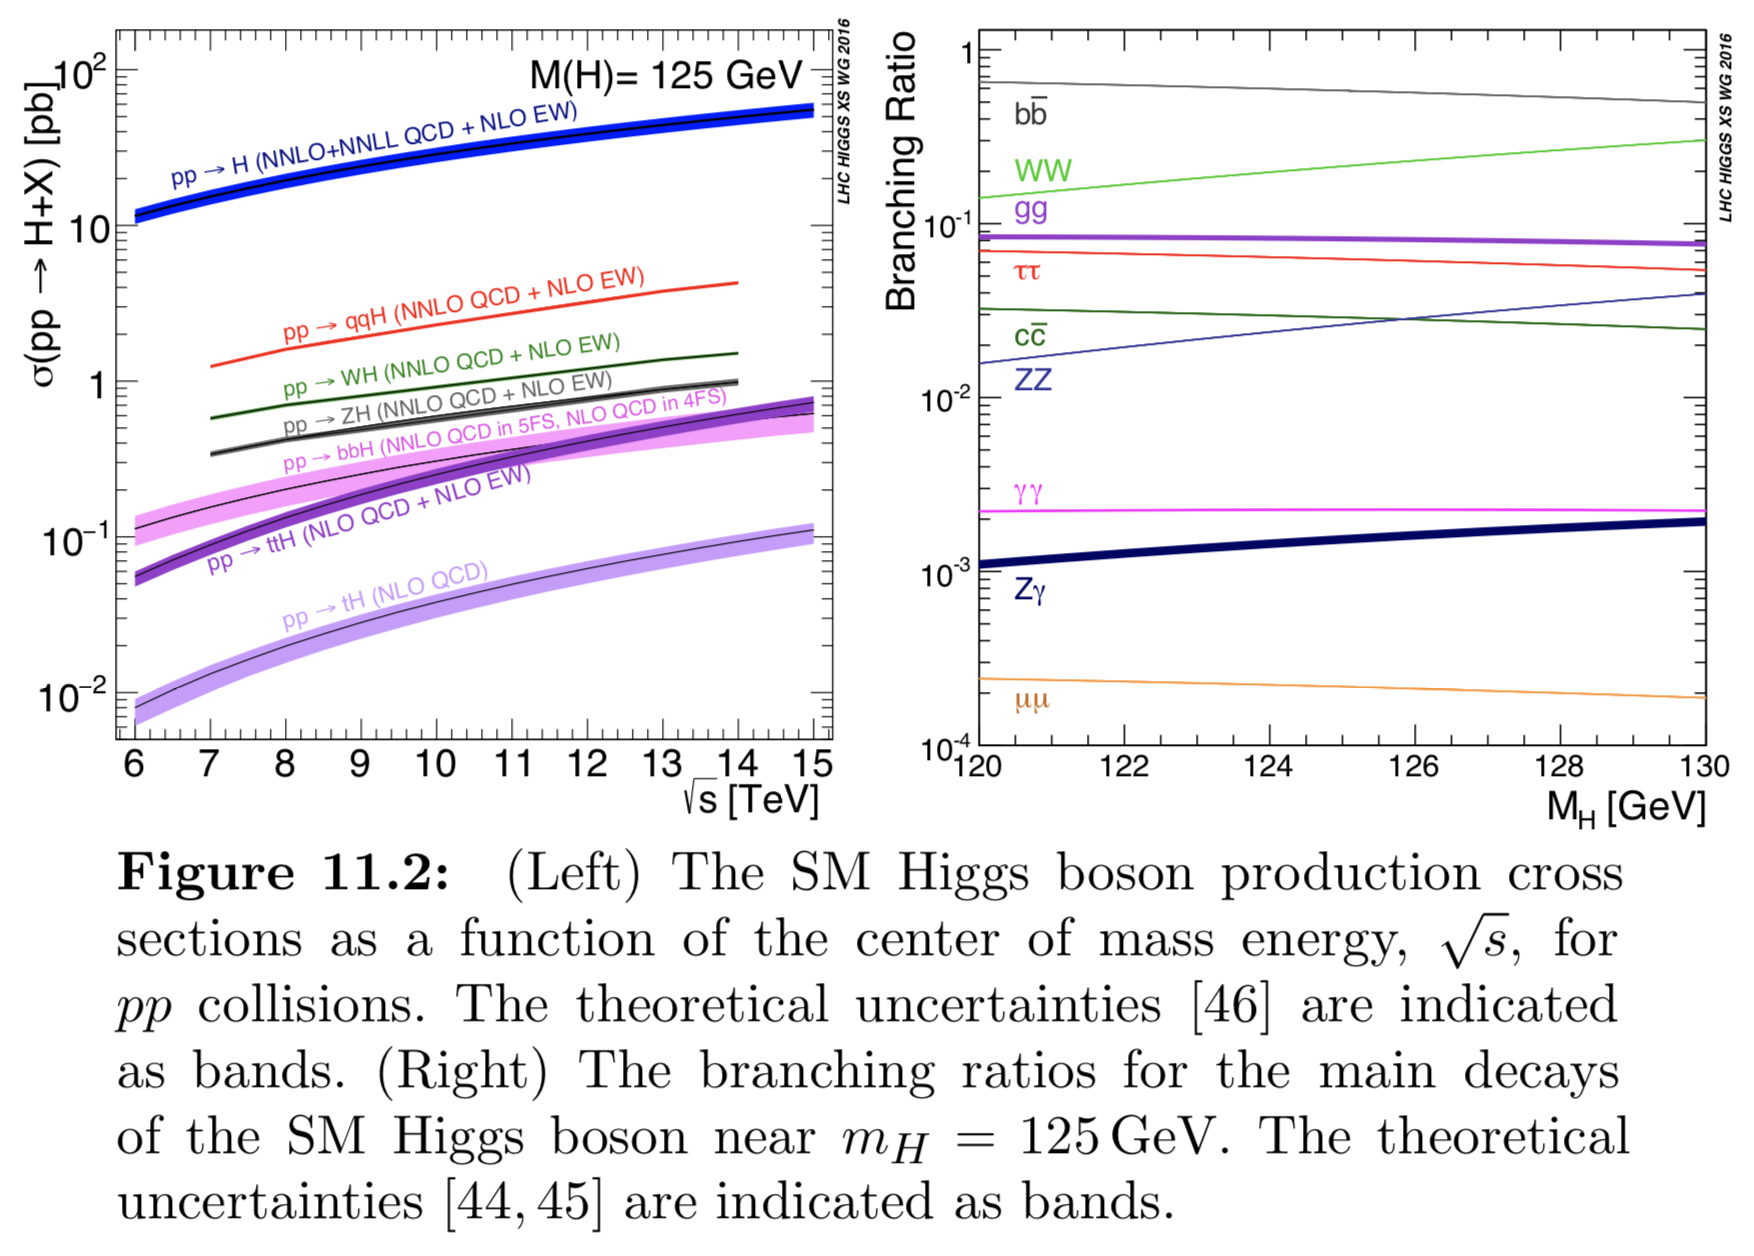
\includegraphics[scale=0.4]{physics/images/higgs_cross_sections}
\end{center}
Consulting the plot on the right, note that the five sets of Higgs final states mentioned before are not the 5 sets with the highest branching ratios for Higgs decays. This is because backgrounds must be considered; the aforementioned five final states are those best optimized to isolate the signals from LHC backgrounds.

On theoretical grounds, for a given $m_H$, the sensitivity of a search channel depends on the production cross section, the branching ratio, the mass resolution, and the backgrounds. For a low-mass Higgs ($110<m_H\text{ (GeV)}<150$), the mass resolutions for the five most important channels are presented in the following table from the PDG:

\begin{center}
    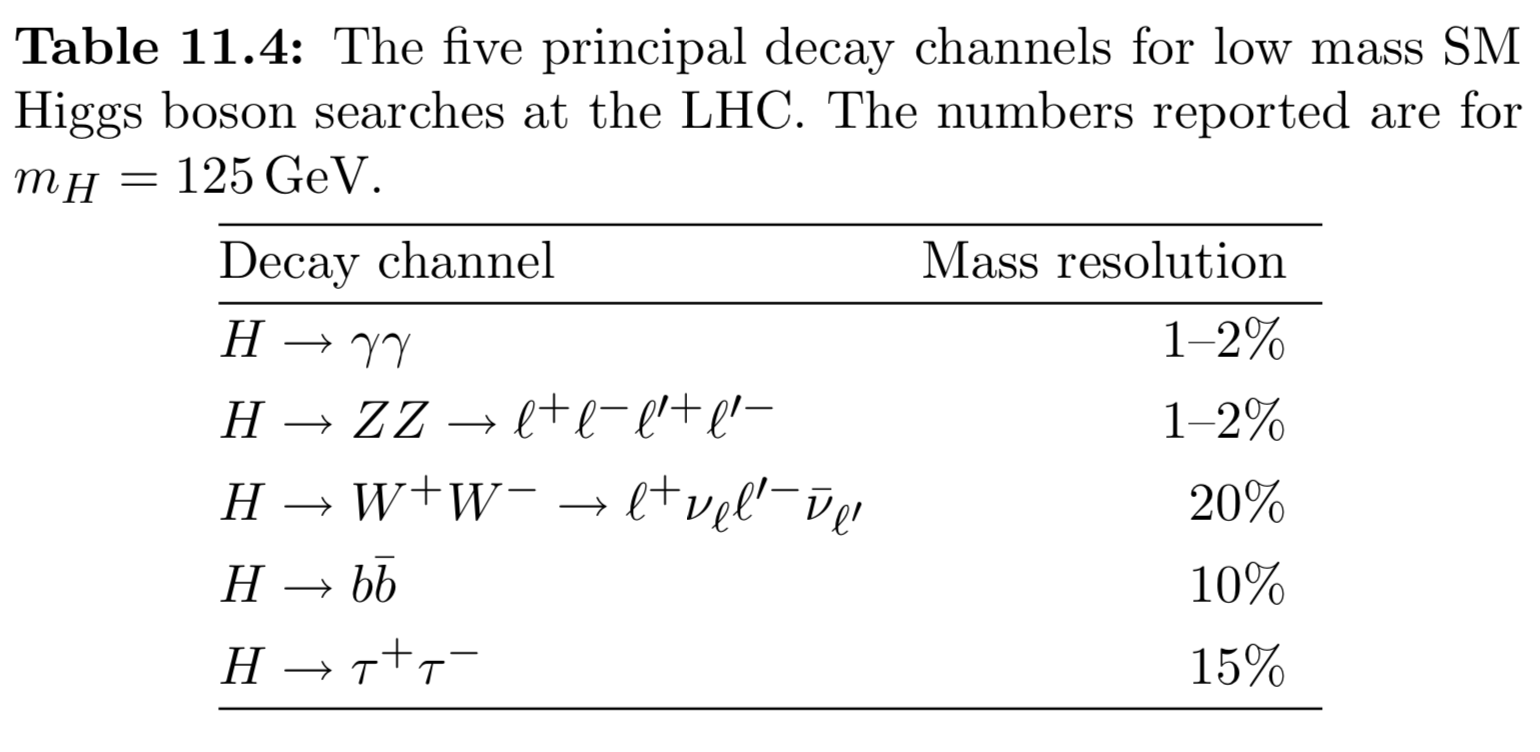
\includegraphics[scale=0.4]{physics/images/higgs_mass_resolution}
\end{center}
When all factors that contribute to a search's sensitivity are considered, $H\rightarrow \gamma \gamma$ and $H\rightarrow ZZ^*\rightarrow 4\ell$ are the best channels for discovery, with excellent mass resolution, well-reducible backgrounds, and precise measurement of all final state particles. Following these at low-mass is $H \rightarrow WW^* \rightarrow \ell \nu \ell \nu$, with a large BR but poor mass resolution due to the presence of two neutrinos as MET. After this are $H\rightarrow b\overline{b}$ and $H\rightarrow \tau \tau$, which have large backgrounds and poor mass resolution.

\vspace{1em}
\vspace{1em}
\noindent \underline{$H \rightarrow \gamma \gamma$}

\vspace{1em}
\noindent A search was performed for a narrow peak over a smoothly falling background in the high $p_T$ diphoton invariant mass distribution $m_{\gamma \gamma}$. The backgrounds are comprised of prompt diphoton, gamma+jets, and dijet processes and are not overwhelming in light of a signal search. To further enhance search sensitivity, events are categorized based on production mechanism: events with high $p_T$ leptons and/or MET consistent with a $W$ or $Z$ decay are tagged in the $VH$ category. Events with diets and a large mass and $\eta$ difference belong to VBF, while remaining events are considered as $VH$ if the jets are compatible with a hadronic $W$ or $Z$, or as GF. The leptonic $VH$ category is quite pure, while VBF has contamination from GF.

\vspace{1em}
\noindent \underline{$H \rightarrow ZZ^* \rightarrow 4l$}

\vspace{1em}
\noindent A search was performed for a narrow peak over a small continuous background dominated by non-resonant $ZZ^*$ production from $qq$ annihilation or $gg$ fusion. Subdominant and reducible backgrounds are $Z+b \overline{b}$, $Z$+jets, and $t \overline{t}$. Lepton isolation and IP cuts are used to suppress these bkg channels. Since the mass resolution and bkg levels are different for the 4$\mu$, 4$e$ and 2$e$ 2$\mu$ subchannels, events are analyzed separately based on the final state leptons and then combined. Furthermore, events are categorized by production mechanism using the same identifiers in the diphoton search.

\vspace{1em}
\noindent Given that we have a 2$e$2$\mu$ event, we prefer to have $Z \rightarrow ee$ and $Z^* \rightarrow \mu \mu$. It is known that the resolutions for detecting both particles follow:


\begin{equation}
\frac{\delta p_T}{p_t} \sim p_T \quad \text{(muons)} \qquad \qquad \
\frac{\delta E}{E} \sim \frac{1}{\sqrt{E}} \quad \text{(electrons)}
\end{equation}
From this, we conclude that we desire lower energy muons so that we may better measure their curvature (and thus $p_T$) and higher energy electrons for better resolution.

\vspace{1em}
\noindent \underline{$H \rightarrow W^+W^- \rightarrow l \nu l \nu$}

\vspace{1em}
\noindent While the production rate is large, the mass resolution is poor due to two neutrinos, and the backgrounds are numerous. Events are divided based on the lepton flavor combination and the number of jets. Background reduction and estimation is vital in this search. For events with opposite-flavor lepton and no accompanying high $p_T$ jets, the dominant background stems from non-resonant $WW$ production. Events with same flavor leptons have large Drell-Yan contamination. $Wt$, $W$+jets (with jet misidentified as a lepton), and $t\overline{t}$ contaminate all categories \cite{bstone}.

\chapter{Experimental Particle Physics}
Difference between radiation length $\chi_0$ and stopping power $dE/dx$

\section{Passage of Particles through Matter}

A muon is minimum ionizing from $0.1\le \beta\gamma \le 1000$ or equivalently $10$ MeV $\le p\le 100$ GeV. A minimum ionizing muon typically loses 2 MeV $cm^2/g$ through a material. Some typical materials

\begin{center}
    \begin{tabular}{ | c | c| c |} 
        \hline
        Material & Density (g/cm$^3$) & MIP Energy Loss \\ \hline
        Iron & 8 & 16 GeV/m \\
        Air & 0.00125 & 0.25 MeV / m \\
        \hline
    \end{tabular}
\end{center}


\subsection{Radiation Length}
Characterizes a material. Distance over which 
\begin{itemize}
    \item Electron is reduced to $1/e$ of it's initial energy
    \item 7/9 the mean free path of a photon before it pair produces
\end{itemize}
Typically measured in $g/cm^2$, so need to divide by the density to get the correct value. This is done since the density of a material is variable.

\begin{center}
    \begin{tabular}{ | c | c|} 
        \hline
        Material & $X_0$ (cm) \\ \hline
        Iron & 1.75 \\
        Lead Tungstate & 0.89 \\
        Water & 36.08 \\
        Air & 30.39 \\
        \hline
    \end{tabular}
\end{center}



\subsection{Multiple Scattering}
For relativistic particles, the angle $\theta$ scattered in a material is
\begin{align}
\theta \approx \frac{13.6 \textrm{MeV}}{\beta c p}z\sqrt{\frac{X}{X_0}}
\end{align}
Where $p,z$ is the momentum and charge respectively of the incident particle. $X$ is the distance travelled in the medium with radiation length $X_0$. Becomes less and less relevant as particle momentum increases (depends on $1/p$)

\subsection{Bremsstrahlung}
 An electron loses most of its energy through Bremsstrahlung at energies $\ge 10$ MeV. Electron energy loss by Brem $\propto E_e$, loss by ionization $\propto \ln E_e$. Shower length is roughly twice that of the radiation length of a material \cite{pdg} The critical energy of a muon in Iron (i.e. the energy at which Radiative losses are equal to Ionization losses) is $E_{\mu c} = 332$ GeV. Muon energy loss goes as 
 \begin{align}
 -dE/dx = a(E) + b(E)E
 \end{align}
 $a(E)\approx 0.002$ g$^{-1}$cm$^2$ is from ionization energy loss, $b(E)$ is from brem, pair production, etc.
\subsection{Cascade Showers}

Electromagnetic showers caused by Bremstrallung which creates high energy photon, which then pair produces, and the products of which then brem high energy photons, etc until everything is out of energy.

Transverse development of a shower is parametrized by the Moliere radius $R_M$


\begin{align}
R_M = X_0E_s/E_c
\end{align}

Electrons only? $E_s = 21$ MeV is the "scale" energy? Only 10$\%$ of the energy lies outside of the cylinder of this size, $99\%$ is within 3.5$R_M$. 

\subsection{Pair Production}
Electron pairs are produced by photons in the electric field created by the nucleus. Pairs take energy, nucleus balances momentum. (Rossi pg. 13)

\subsection{Landau-Pomeranchuk-Migdal (LPM) Effect}
For very high energy particles, neighboring nuclei get squished which causes a suppression of both bremsstrahlung and pair-production.



\section{Symmetries}
\subsection{Parity}
Parity inversion is the flip of the sign of all three spatial coordinates of a system. Effectively what it does is change something into it's mirror image. The symmetry assumes that if the world were actually it's mirror image (i.e. everything that was once "left" becomes "right"), all of the Physics would remain exactly the same. This symmetry can be tested for by looking at the \textbf{helicity} associated with an interaction
\begin{align}
h = \textbf{S}\cdot\textbf{p}
\end{align}
Under parity inversion, the momentum of a particle changes sign (vector), whereas the spin does not (axial vector). This causes the helicity to change sign under parity inversion. If an interaction respects the symmetry of parity inversion, the average of this quantity should come out to be zero, since if it did not, it would imply that the real world, and the "mirror image" world would be different from each other.

Madame Wu led an experiment that looked at beta decays from cold Cobalt-60 atoms which had their spins aligned in a uniform magnetic field. This gave the direction of the $\textbf{S}$ vector used in the Helicity measurement. From here, all that was left to do was measure the direction which the electron was emitted, effectively upwards or downwards relative to the spin of the nucleus. If parity was not violated, helicity should average to zero, which means one should see the same amount going up as down.

The Cobalt subsequently decayed electromagnetically through two $\gamma$'s. The electromagnetic interaction was known to respect parity conservation, so they used the photons to measure how polarized they were able to get the Cobalt atoms initially. The direction of the photons gave the direction of the nuclear spin. If the electron decay was parity invariant, the electrons should be found on average to have no correlation with the direction of the emitted photons. It was found that they tracked exactly opposite this direction revealing the weak force to \emph{maximally} violate parity.

\begin{align}
\langle h \rangle = \langle \textbf{S}\cdot\textbf{p} \rangle \neq 0
\end{align}

For a massive particle, the helicity is not Lorentz invariant, since it is always possible to boost to a frame in which the momentum vector changes, while the direction of spin does not. The \textbf{chirality} of a particle tells us how a particle transforms in the right- or left-handed representation of the Poincare group. For massless particles this is the same as helicity, but is different for things with mass. Only left-handed fermions and right-handed antifermions interact with the weak-interaction.



\section{Experimental Conservation Laws}

\begin{itemize}
    \item Conservation of Charge - 
    \item Conservation of Leptons - Amount of electrons, muons, taus always conserved, keeping count with neutrinos, etc.
    \item Conservation of Color - At a strong vertex the quark color changes (there are three), the difference is carried by the gluon.
    \item Conservation of Baryon number - amount of quarks are always conserved. Cabbibo mixing lets quarks change generations
    \item $\sim$ Conservation of Flavor - not a real conservation law, but mostly true, conserved in strong and electromagnetic decays, not weak decays
\end{itemize}
Lepton number is conserved because...

Spin affects particle decays, if a spin-0 particle decays, it is isotropic. Weak decays, since they violate parity, decay preferentially in the direction along the axis of their momentum (?)


Most of the time, lepton flavor is conserved except in neutrino oscillations.

\section{Particle Detection}
\subsection{Cherenkov Radiation}
Happens when a particle travels faster than the speed of light does within a particular medium. It is characterized by a "cone" which makes a angle dependent on the speed of the particle producing the light
\begin{align}
\cos\theta =\frac{1}{n\beta}
\end{align}
Where $n$ is the index of refraction of the medium, and $\beta = v/c$ of the particle.


\section{Cross Section and Luminosity}
First we define the instantaneous luminosity (typically just called the \textbf{luminosity}) of a beam of particles as \cite{cousins}
\begin{align}
\mathcal{L} = \textrm{number~of~incident~particles~per~unit~area,~per~unit~time}
\end{align}

We use this as a metric for how much beam we have. We don't just want the number of particles per unit time because it wouldn't tell us how concentrated our beam is.  Typical values of the instantaneous LHC (circa August 2018) are
\begin{align}
\mathcal{L}_{LHC} &\approx 2\times 10^{38} /m^2s
\end{align}
To get an understanding of this number, the diameter of a human hair is roughly  100 $\mu m$, so
\begin{align}
\textrm{cross section of human hair} \approx   10^4 \mu m^2
\end{align}
A mole of atoms is of course $10^{23}$, so putting it all together
\begin{align}
\mathcal{L}_{LHC} \approx 20 \textrm{~moles / hair~} \mu s
\end{align}
We are shooting about 20 moles worth of protons through an area the size of a human hair every microsecond.

When we shoot two beams together, or a beam at a wall, we generally care about how many of these particles (per unit time) get scattered, i.e smash into each other and go flying off. We write this value as $dN/dt$ and is related to the instantaneous luminosity with

\begin{align}
\frac{dN}{dt} = \sigma\mathcal{L}
\end{align}
Where $\sigma$ is called the \textbf{cross section} for the collision to occur, having units of area. The larger the cross section, the more scattered particles you will get. In actuality, one counts how many scattered particles show up at each angle, giving us a differential $\sigma$, which is then integrated over all angles to get the full cross section \cite{griffiths_qm}.


Another common value is the \textbf{integrated luminosity} which is simply the instantaneous luminosity added up over some period of time. With this, we can calculate how many scattered particles we had over a given time
\begin{align}
N = \sigma \int \mathcal{L}~dt
\end{align}

Integrated luminosity effectively tells us how many particles have passed through the collision point.  Units are inverse "barns" (1 barn = 100 fm$^2$), which was supposed to be a large area (size of a typical nucleus) concerning nuclear interactions. Integrated luminosity tells us, if we were to put all the particles that passed through the interaction point all there at once, how dense the plane would be filled with these particles. As you increase integrated luminosity, you decrease the scale (i.e. $pb^{-1} \rightarrow fb^{-1}$) which shows that the density of particles is increasing. Integrated luminosity of the LHC is given as

\begin{center}
\begin{tabular}{ | c | c|} 
\hline
 Year & $\int \mathcal{L} dt$ [$fb^{-1}$] \\ \hline
 2018 & 67.86  \\ 
 2017 & 49.79  \\
2016 & 37.80   \\ 
2015 & 4.21 \\
2012 & 21.79 \\
2011 & 5.55\\
\hline
\end{tabular}
\end{center}

\section{Famous Experiments}

\subsection{LEP}\label{lep}
The Large Electron Positron Collider was used 1989-2000 at CERN. With an energy of 209 GeV, was used for precision data on the $Z$ and $W$ boson. It was a circular collider with a 27 km circumference.
\subsection{CDF}
Proton-antiproton collider at Fermilab (Collider Detector at Fermilab). Got to about $2$ TeV center of mass energy, was where the top quark was discovered.

\subsection{CMS}


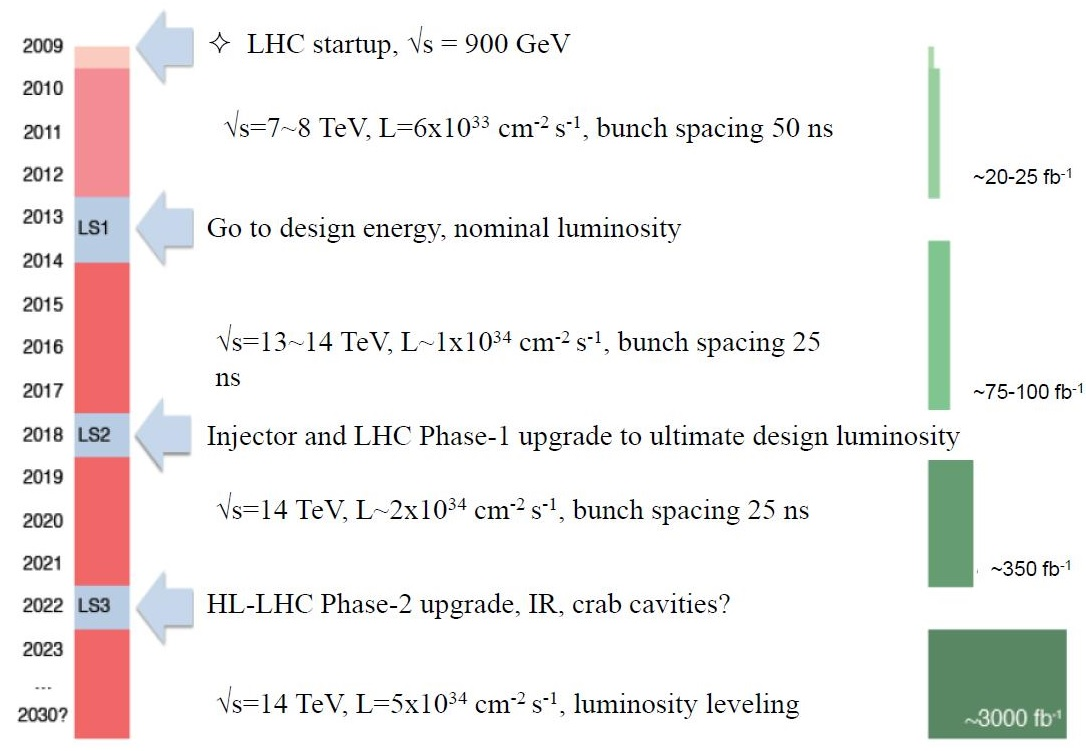
\includegraphics[width=1.0\textwidth]{physics/images/lhc_timeline}


\subsection{Types of Searches}
\begin{itemize}
    \item Long lived neutral particles that decay into muons (detected in muon system, but have displaced vertex)
    \item Long lived charge particles, if they have a large mass, will go slower, can detect through timing (takes longer to get to muon system)
\end{itemize}

\subsection{Pseudorapidity}
The pseudorapidity $\eta$ is used in CMS as a coordinate that directly maps to the angle $\theta$ of a particle relative to the beam line.
\begin{align}
\eta = -\ln\left[\tan\frac{\theta}{2}\right]
\end{align}
It is useful because particle production is large closer to the beam line, and slices of $\eta$ are roughly equally populated whereas slices of $\theta$ are not. Additionally differences in $\eta$ are Lorentz invariant.
